%%%%%%%%%%%%%%%%%%%%%%%%%%%%%%%%%%%%%%%%%%%%%%%%%%%%%%%%%%%%%%%%%%
%%%%%%%%%%%%%%%%%%%%%%%%%%%%%%%%%%%%%%%%%%%%%%%%%%%%%%%%%%%%%%%%%%
%Packages
\documentclass[10pt, a4paper]{article}
\usepackage[top=3cm, bottom=4cm, left=3.5cm, right=3.5cm]{geometry}
\usepackage{amsmath,amsthm,amsfonts,amssymb,amscd, fancyhdr, color, comment, graphicx, environ}
\usepackage{float}
\usepackage{mathrsfs}
\usepackage[math-style=ISO]{unicode-math}
\setmathfont{TeX Gyre Termes Math}
\usepackage{lastpage}
\usepackage[dvipsnames]{xcolor}
\usepackage[framemethod=TikZ]{mdframed}
\usepackage{enumerate}
\usepackage[shortlabels]{enumitem}
\usepackage{fancyhdr}
\usepackage{indentfirst}
\usepackage{listings}
\usepackage{sectsty}
\usepackage{thmtools}
\usepackage{shadethm}
\usepackage{hyperref}
\usepackage{setspace}
\usepackage[linguistics]{forest}
\hypersetup{
    colorlinks=true,
    linkcolor=blue,
    filecolor=magenta,      
    urlcolor=blue,
}
%%%%%%%%%%%%%%%%%%%%%%%%%%%%%%%%%%%%%%%%%%%%%%%%%%%%%%%%%%%%%%%%%%
%%%%%%%%%%%%%%%%%%%%%%%%%%%%%%%%%%%%%%%%%%%%%%%%%%%%%%%%%%%%%%%%%%
%Environment setup
\mdfsetup{skipabove=\topskip,skipbelow=\topskip}
\newrobustcmd\ExampleText{%
An \textit{inhomogeneous linear} differential equation has the form
\begin{align}
L[v ] = f,
\end{align}
where $L$ is a linear differential operator, $v$ is the dependent
variable, and $f$ is a given non−zero function of the independent
variables alone.
}
\mdfdefinestyle{theoremstyle}{%
linecolor=black,linewidth=1pt,%
frametitlerule=true,%
frametitlebackgroundcolor=gray!20,
innertopmargin=\topskip,
}
\mdtheorem[style=theoremstyle]{Problem}{Problem}
\newenvironment{Solution}{\textbf{Solution.}}

\definecolor{codegreen}{rgb}{0,0.6,0}
\definecolor{codegray}{rgb}{0.5,0.5,0.5}
\definecolor{codepurple}{rgb}{0.58,0,0.82}
\definecolor{backcolour}{rgb}{0.95,0.95,0.92}

\lstdefinestyle{mystyle}{
    backgroundcolor=\color{backcolour},   
    commentstyle=\color{codegreen},
    keywordstyle=\color{magenta},
    numberstyle=\tiny\color{codegray},
    stringstyle=\color{codepurple},
    basicstyle=\ttfamily\footnotesize,
    breakatwhitespace=false,         
    breaklines=true,                 
    captionpos=b,                    
    keepspaces=true,                 
    numbers=left,                    
    numbersep=5pt,                  
    showspaces=false,                
    showstringspaces=false,
    showtabs=false,                  
    tabsize=2
}

\lstset{style=mystyle}
%%%%%%%%%%%%%%%%%%%%%%%%%%%%%%%%%%%%%%%%%%%%%%%%%%%%%%%%%%%%%%%%%%
%%%%%%%%%%%%%%%%%%%%%%%%%%%%%%%%%%%%%%%%%%%%%%%%%%%%%%%%%%%%%%%%%%
%Fill in the appropriate information below
\newcommand{\norm}[1]{\left\lVert#1\right\rVert}     
\newcommand\course{EES405}                            % <-- course name   
\newcommand\hwnumber{Lab Assignment-01}                                 % <-- homework number
\newcommand\Information{(Shiv Shankar Singh)}% <-- personal information
\newcommand\Roll{(MS18006)}
%%%%%%%%%%%%%%%%%%%%%%%%%%%%%%%%%%%%%%%%%%%%%%%%%%%%%%%%%%%%%%%%%%
%%%%%%%%%%%%%%%%%%%%%%%%%%%%%%%%%%%%%%%%%%%%%%%%%%%%%%%%%%%%%%%%%%
%Page setup
\pagestyle{fancy}
\headheight 35pt
\lhead{\today}
\rhead{
\includegraphics[width=2.5cm]{iisermlogo.jpg}}
\lfoot{}
\pagenumbering{arabic}
\cfoot{\small\thepage}
\rfoot{}
\headsep 1.2em
\renewcommand{\baselinestretch}{1.25}
%%%%%%%%%%%%%%%%%%%%%%%%%%%%%%%%%%%%%%%%%%%%%%%%%%%%%%%%%%%%%%%%%%
%%%%%%%%%%%%%%%%%%%%%%%%%%%%%%%%%%%%%%%%%%%%%%%%%%%%%%%%%%%%%%%%%%
%Add new commands here
\renewcommand{\labelenumi}{\alph{enumi})}
\newcommand{\Z}{\mathbb Z}
\newcommand{\R}{\mathbb R}
\newcommand{\Q}{\mathbb Q}
\newcommand{\NN}{\mathbb N}
\newcommand{\PP}{\mathbb P}
\DeclareMathOperator{\Mod}{Mod} 
\renewcommand\lstlistingname{Algorithm}
\renewcommand\lstlistlistingname{Algorithms}
\def\lstlistingautorefname{Alg.}
\newtheorem*{theorem}{Theorem}
\newtheorem*{lemma}{Lemma}
\newtheorem{case}{Case}
\newcommand{\assign}{:=}
\newcommand{\infixiff}{\text{ iff }}
\newcommand{\nobracket}{}
\newcommand{\backassign}{=:}
\newcommand{\tmmathbf}[1]{\ensuremath{\boldsymbol{#1}}}
\newcommand{\tmop}[1]{\ensuremath{\operatorname{#1}}}
\newcommand{\tmtextbf}[1]{\text{{\bfseries{#1}}}}
\newcommand{\tmtextit}[1]{\text{{\itshape{#1}}}}

\newenvironment{itemizedot}{\begin{itemize} \renewcommand{\labelitemi}{$\bullet$}\renewcommand{\labelitemii}{$\bullet$}\renewcommand{\labelitemiii}{$\bullet$}\renewcommand{\labelitemiv}{$\bullet$}}{\end{itemize}}
\catcode`\<=\active \def<{
\fontencoding{T1}\selectfont\symbol{60}\fontencoding{\encodingdefault}}
\catcode`\>=\active \def>{
\fontencoding{T1}\selectfont\symbol{62}\fontencoding{\encodingdefault}}
\catcode`\<=\active \def<{
\fontencoding{T1}\selectfont\symbol{60}\fontencoding{\encodingdefault}}

%%%%%%%%%%%%%%%%%%%%%%%%%%%%%%%%%%%%%%%%%%%%%%%%%%%%%%%%%%%%%%%%%%
%%%%%%%%%%%%%%%%%%%%%%%%%%%%%%%%%%%%%%%%%%%%%%%%%%%%%%%%%%%%%%%%%%
%Begin now!



\begin{document}

\begin{titlepage}
    \begin{center}
        \vspace*{3cm}
            
        \Huge
        \textbf{Climate Data Analysis}
            
        \vspace{1cm}
        \huge
        \hwnumber
            
        \vspace{1.5cm}
        \Large
            
        \textbf{\Information}                      % <-- author
        
            
        \vfill
        
        \course
            
        \vspace{1cm}
            
        
\includegraphics[width=0.4\textwidth]{iisermlogo.jpg}
        \\
        
        \Large
        
        \today
            
    \end{center}
\end{titlepage}

%%%%%%%%%%%%%%%%%%%%%%%%%%%%%%%%%%%%%%%%%%%%%%%%%%%%%%%%%%%%%%%%%%
%%%%%%%%%%%%%%%%%%%%%%%%%%%%%%%%%%%%%%%%%%%%%%%%%%%%%%%%%%%%%%%%%%
%Start the assignment now
%%%%%%%%%%%%%%%%%%%%%%%%%%%%%%%%%%%%%%%%%%%%%%%%%%%%%%%%%%%%%%%%%%
%New problem
\newpage
Lab Assignment-01
\subsubsection*{Plot vertical thermal structure of the atmosphere using NCEP/NCAR long-term mean data for summer (JJAS mean), winter (DJF mean) and annual (mean of Jan-Dec) using Python.}

\begin{Problem}
\begin{enumerate}
    \item Vertical Thermal structure of the Globe (0-360E $\&$  90S – 90N)
    \item Vertical Thermal structure of the Tropics (0-360E $\&$ 30S – 30N)
    \item Vertical Thermal structure of the North Pole (0-360E $\&$ 70N – 90N)
    \item Vertical Thermal structure over India (60-110E $\&$ 6N – 35N)
\end{enumerate}
\end{Problem}

\begin{Solution}

% Example of a lemma.
% \begin{lemma}
%     This is a lemma.
% \end{lemma}

% Example of a proof.
% \begin{proof}
%     Write your proof here.
% \end{proof}

% Example of including a picture.
% \begin{center}
%     
\includegraphics[width = 4cm]{iisermlogo.jpg}
% \end{center}

% Example of referring to a piece of code.
% \lstinputlisting[language = python]{Program Solution.py}

% Example of a table.
% \begin{equation*}\begin{tabular}{ c c c }
%                 & Mean          & SD \\ 
%      Fall 2077  & 7.046512      & 1.714552 \\  
%      Fall 1977  & 9.102941      & 1.568919
% \end{tabular}\end{equation*}

% Overall, this is a quite basic template for assignments, and above are only some basic features. I included enough packages and set a few environments. You may modify them or add features to fit your personal preference. Enjoy using it!

I plotted the vertical thermal structure of different regions (Globally, Tropics (-30,30), North Pole (70,90) and India) across three different seasons (Summer (JJAS), winter (DJF), and annual mean). \\
I followed the following protocol/steps in generating all the above plots. \\

\begin{enumerate}
    \item \textbf{Step:1} Load the data in an array format with xarray library
    \item \textbf{Step:2} Take mean of the data along latitude, longitude and time axis 
    \item \textbf{Step:3} Generate plot with data.mean along x-axis and pressure levels along y-axis
    \end{enumerate}
For python source code to execute the above task, see Appendix.\\
\subsection*{Plots generated}
% Vertical thermal structure of different regions across seasons
\subsubsection{Vertical Thermal structure over India (60-110E $\&$ 6N – 35N)}

\begin{figure}[b]
    \centering
    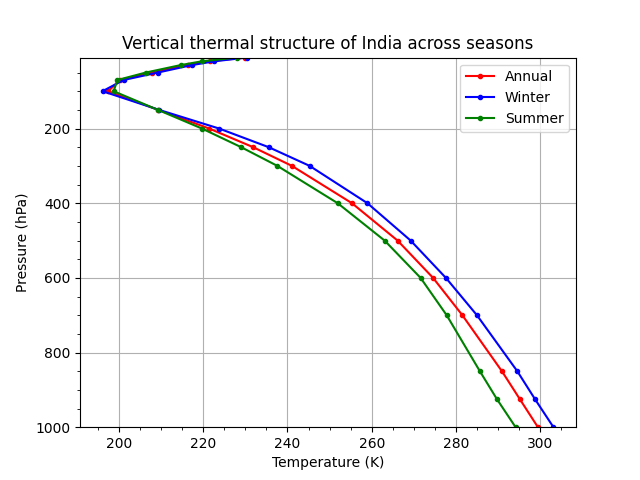
\includegraphics[width=0.33\textwidth]{india_seasons.png}
    \caption{Vertical Thermal structure over India (60-110E $\&$ 6N – 35N)}
    \label{fig:my_label}
\end{figure}
Here, we can see that there are almost no changes in the vertical thermal structure going up into the atmosphere, as India lies in the tropical region. The convection setup helps in the regulation of the temperature profile across seasons.

\newpage
Lab Assignment-01
\subsubsection{Vertical thermal structure of Tropics (0-360 $\&$ 30S-30N)}
As expected, since the tropics receive the same amount of sunlight throughout the year and there are no significant changes in the solar flux received across the seasons, hence the vertical temperature profile is almost the same across the seasons.
\begin{figure}[h]
    \centering
    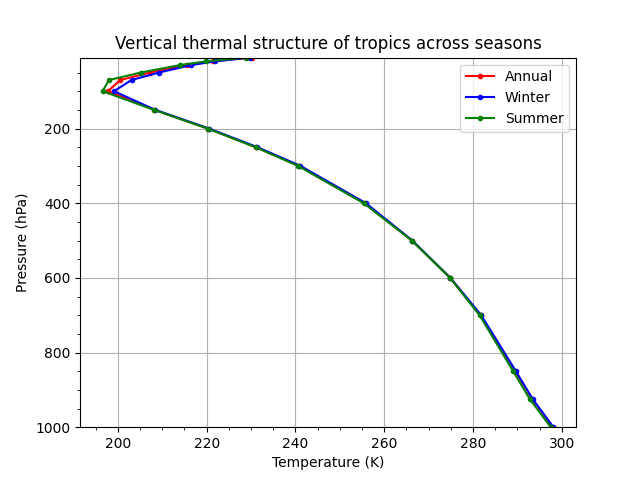
\includegraphics[width=0.5\textwidth]{tropics_seasons.png}
    \caption{Vertical thermal structure of Tropics (0-360 $\&$ 30S-30N)}
    \label{fig:my_label}
\end{figure}

\subsubsection{Vertical thermal structure of North Pole (0-360 $\&$ 70N-90N)}

Since, the amount of sunlight received by the north pole varies drastically across seasons, the same can be inferred from vertical thermal structure over north pole, where we can see that the profiles of different seasons(summer and winter) are quite spread apart from each other.

\begin{figure}[h]
    \centering
    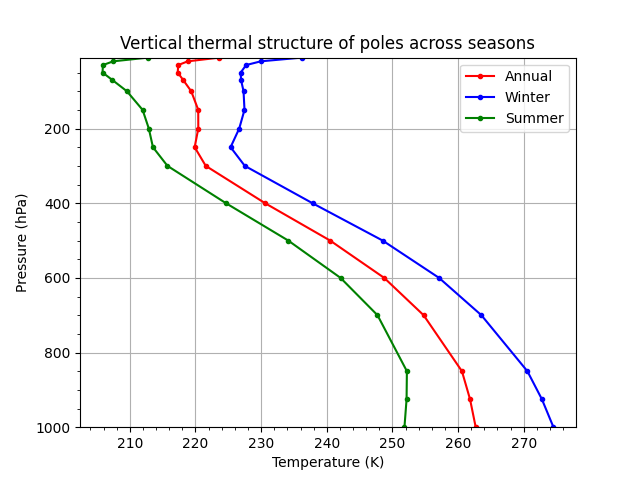
\includegraphics[width=0.5\textwidth]{poles_seasons.png}
    \caption{Vertical thermal structure of North Pole (0-360 $\&$ 70N-90N)}
    \label{fig:my_label}
\end{figure}

\newpage
Lab Assignment-01
\subsubsection{Vertical thermal structure of globe}
The vertical thermal profile averaged over the whole of the globe doesn't seem to vary much as the annual budget of sunlight received doesn't change across the seasons (summer in the northern hemisphere is compensated by winter in the southern hemisphere and vice versa) as it is averaged over the entire globe.
\begin{figure}[h]
    \centering
    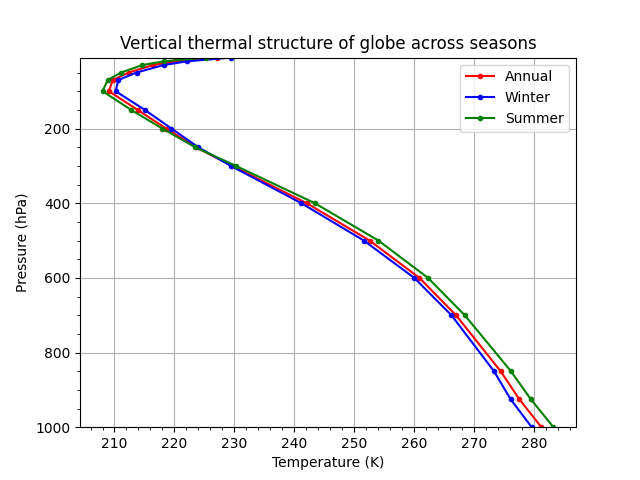
\includegraphics[width=0.5\textwidth]{global_seasons.png}
    \caption{Caption}
    \label{fig:my_label}
\end{figure}


\end{Solution}

%%%%%%%%%%%%%%%%%%%%%%%%%%%%%%%%%%%%%%%%%%%%%%%%%%%%%%%%%%%%%%%%%%
%Complete the assignment now
\end{document}

%%%%%%%%%%%%%%%%%%%%%%%%%%%%%%%%%%%%%%%%%%%%%%%%%%%%%%%%%%%%%%%%%%
%%%%%%%%%%%%%%%%%%%%%%%%%%%%%%%%%%%%%%%%%%%%%%%%%%%%%%%%%%%%%%%%%%
